\usetikzlibrary{arrows}

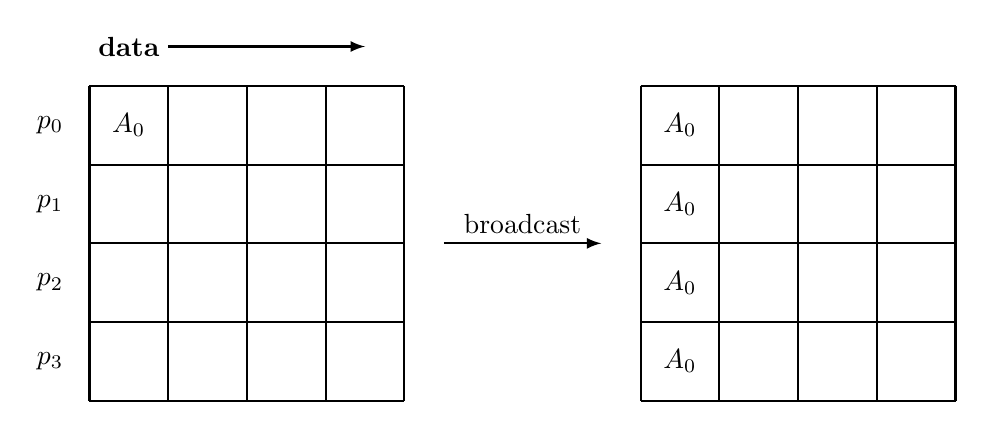
\begin{tikzpicture}

\draw[thick] (0,0) grid +(4,4);

\node at (0.5,3.5) {$A_0$};

\node at (0.5,4.5) {\bf data};
\draw [thick, -latex](1,4.5) -- (3.5,4.5);

\node at (-0.5,3.5) {$p_0$};
\node at (-0.5,2.5) {$p_1$};
\node at (-0.5,1.5) {$p_2$};
\node at (-0.5,0.5) {$p_3$};

\node at (5.5, 2.25){broadcast}; 
\draw [thick, -latex](4.5,2) -- (6.5,2);

\draw[thick] (7,0) grid +(4,4);

\node at (7.5,0.5) {$A_0$};
\node at (7.5,1.5) {$A_0$};
\node at (7.5,2.5) {$A_0$};
\node at (7.5,3.5) {$A_0$};


\end{tikzpicture}